\bigskip
Debido a que la volatilidad varía através del tiempo en  los retornos de Netflix, los modelos clásicos de series de tiempo como los \textit{Arima } o \textit{ARMA} no son adecuados para modelarla, ya que una de las premisas es que la varianza es constante.

\begin{figure}[!ht]
    \centering
    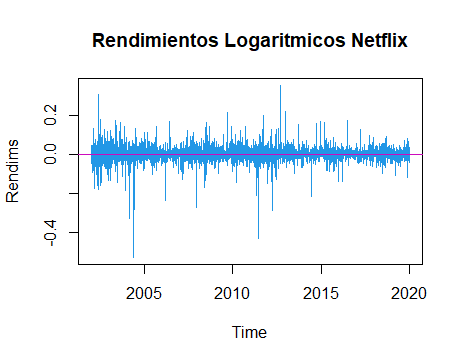
\includegraphics[scale=.75]{Graficos/RendimientosLog.png}
    \caption{Rendimientos Logaritmicos}
    \label{Rendimientos Logaritmicos}
\end{figure}

Notemos que esta serie no tiene tendencia, los valores oscilan alrededor del 0 y además es fácil ver que la variabilidad va cambiando, se presenta períodos largos de alta volatilidad seguidos por períodos de baja volatilidad, lo que indica \textbf{apriori} la presencia de heterocedasticidad. Para comprobar este hecho, miraremos las gráficas de las funciones de auto correlación y auto correlación parcial, tanto de la serie como la del cuadrado de esta, para comprobar que no existe correlación de primer orden, pero si de orden cuadrático. Como se puede comprobar en la gráfica \ref{ACF}.


\begin{figure}[ht]
    \centering
    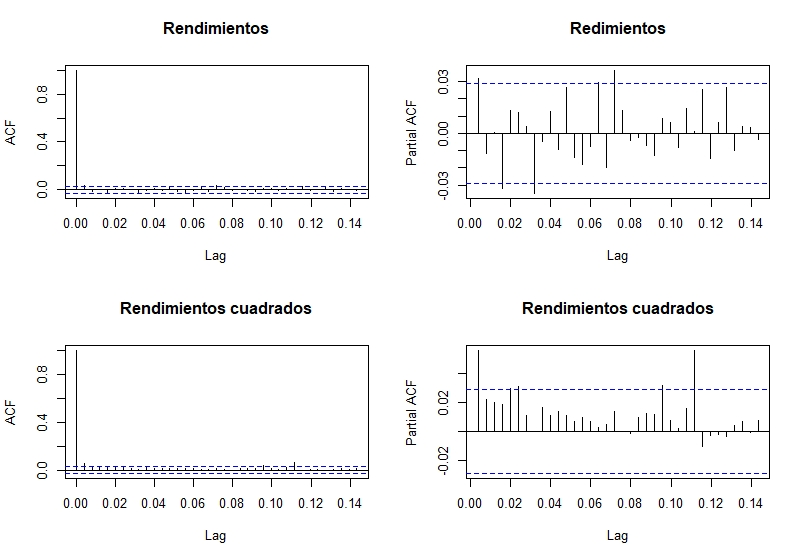
\includegraphics[width=0.75\textwidth]{Graficos/ACFRendi.jpeg}
    \caption{Correlogramas}
    \label{ACF}
\end{figure}


\newpage

Es por ello que se decidió modelar nuestros rendimientos con un \textit{modelo generalizado, auto-regresivo, condicionalmente heterocedástico} que por sus siglas en ingles se denota
\textbf{GARCH(q,p)}
\newline Decimos que es: 

\begin{itemize}
\item Generalizado: Ya que toma en cuenta tanto las observaciones recientes como las históricas.
\item  Autorregresivo: Ya que la variable dependiente se regresa en sí misma.
\item  Condicional: La varianza futura depende de la varianza histórica.
\item Heterocedástico: La varianza cambia en función de las observaciones.
\end{itemize}






En otras palabras, el modelo \textbf{GARCH} encuentra la volatilidad promedio a medio plazo mediante una autorregresión que depende de la suma de los errores retrasados q periodos y de la suma de varianzas retrasadas p periodos. De tal manera que los modelos GARCH(p,q) modelan la volatilidad de la siguiente forma:

\begin{equation}
   \sigma_t^2 =\omega+   \sum^p_{p=1}\alpha_p \epsilon_{t-p}^2 +  \sum^q_{q=1}\beta_q \sigma_{t-q}^2
\end{equation}

Por otro lado, al considerar rendimientos logarítmicos, los modelos GARCH nos permiten observarlos mediante la siguiente expresión:

\begin{equation}
   r_t =\mu_t +  \epsilon_t 
\end{equation}

Donde $\epsilon_t  $ recibe el nombre de innovación y puede ser visto como: 

\begin{equation}
   \epsilon_t =\sigma_t\eta_t 
\end{equation}

Siendo $\eta_t  $ una variable a la cual se le asocia una distribución no necesariamente Normal.
A su vez, como $\epsilon_t$ depende 
$\eta_t$, nuestras innovaciones o residuos tendrán asociada de igual forma una distribución que tendremos que intuir a partir del sesgo y las colas de la distribución de nuestros rendimientos.
\bigskip

Antes de comenzar a proponer nuestros posibles modelos, es conveniente hacer un análisis del histograma de los rendimientos para entender su comportamiento. Se puede apreciar en el gráfico \ref{Histograma de Rendimientos} que se presenta una gran concentración de los datos cerca de la media, es decir, la distribución es leptocúrtica y con colas pesadas. Por otro lado presenta un sesgo en los datos, por lo que podríamos pensar que la distribución de los rendimientos se asemeja a una t-student sesgada.
\begin{figure}[ht]
    \centering
    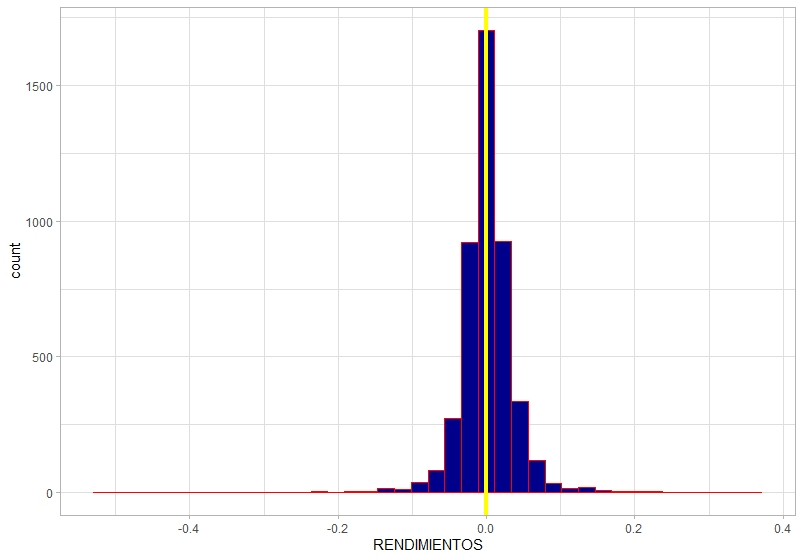
\includegraphics[scale=.5]{Graficos/HistogramaRend.jpeg}
    \caption{Histograma de Rendimientos}
    \label{Histograma de Rendimientos}
\end{figure}

\newpage

Suponiendo dicha distribución, nos dimos a la tarea de probar con distintos modelos GARCH(p,q) suponiendo un modelo autorregresivo de medias móviles para el componente de media observado en la ecuación (2) y modificando los grados de los polinomios de retraso (p y q) asociados a los residuos y a la varianza. 
\bigskip
\smallskip

Nuestro primer criterio para determinar cual es el mejor modelo es encontrar el que tiene el AIC y BIC mas pequeño, pues recordemos que estas pruebas se rigen bajo el principio de parsimonia es decir buscan el modelo mas simple que mejor describa las variables.
\bigskip
En la tabla  \ref{Modelos Propuestos} podemos observar una serie de modelos candidatos que podrian ajustarse a nuestros rendimientos
\input{Tablas/Comparacion de modelo }

Podemos apreciar en la tabla \ref{Modelos Propuestos} que el mejor resulta ser el modelo \textbf{GARCH(1,2)} compuesto con un modelo \textbf{ARMA(1,1)} para el componente de media $\mu_t$, es decir, estamos considerando a los rendimientos de la siguiente forma:

 \begin{equation}
   r_t =  \mu + \phi(r_{t-1} - \mu) + \theta \epsilon_{t-1} +  \epsilon_t
\end{equation}

Donde $\mu$ es una constante a estimar, $\phi$ es el coeficiente del componente autorregresivo AR y $\theta$ es el coeficiente del componente de medias móviles MA.

